\documentclass{article}
\usepackage[T1]{fontenc}
\usepackage{lmodern}
\usepackage{graphicx}
\usepackage{amsmath,amssymb}
\usepackage[a4paper,margin=2cm]{geometry}
\usepackage[absolute,overlay]{textpos}
\setlength{\TPHorizModule}{1mm}
\setlength{\TPVertModule}{1mm}
\usepackage[indonesian]{babel}
\usepackage{hyperref}
\setlength{\emergencystretch}{2em}
% unit: Halaman 81

\begin{document}

% === Halaman 81 (python/native) ===

Step 1: Tentukan parameter masukan (key, nonce, counter)

Step 2: Inisialisasi matriks state berukuran 4 x 4, setiap elemen matriks berukuran 1 

word, 1 word = 32 bit. Total ukuran matriks 16 x 32 bit = 512 bit. State berisi 

konstanta (‘expand 32-byte k’), key, counter, dan nonce dengan pengaturan letak 

sebagai  berikut:

81

Matriks state

Catatan: Di dalam kdoe program, matriks state dinyatakan sebagai sebuah larik in[0..15]

% deskripsi: gambar native xref 320
\noindent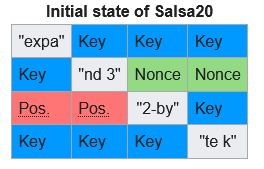
\includegraphics[width=0.85\textwidth]{../../images/python/page_081_img_01.png}

% deskripsi: gambar native xref 321
\noindent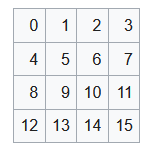
\includegraphics[width=0.85\textwidth]{../../images/python/page_081_img_02.png}

\end{document}
